% Capítulo 6 (Resultados) — Slide 8 — Heatmap CTI por política e POD (figura isolada)
\begin{frame}{CTI médio por política e perfil}
  \centering
  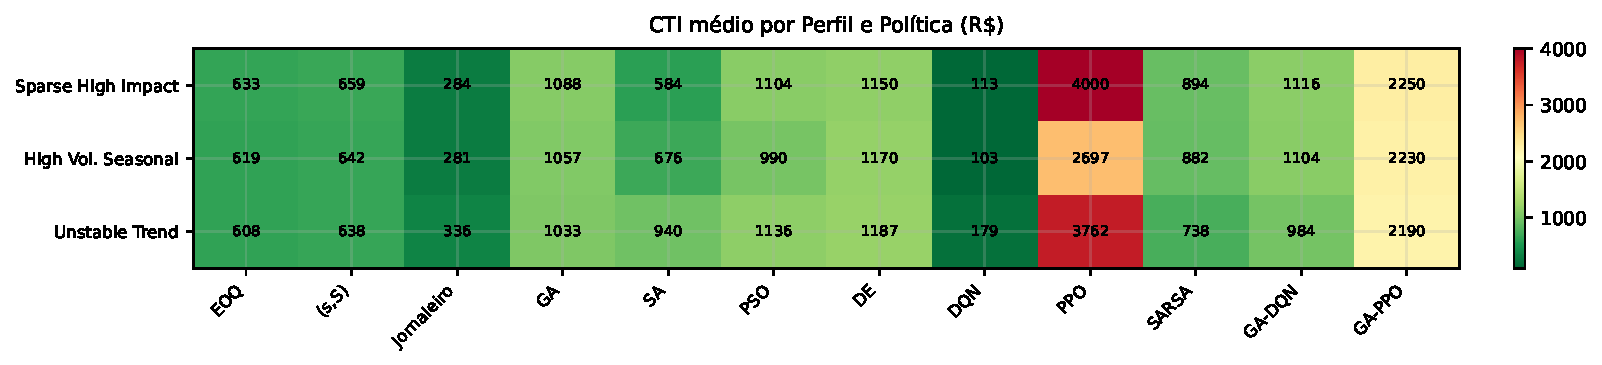
\includegraphics[width=0.82\linewidth,height=6.4cm,keepaspectratio]{figures/profile_policy_heatmap_cti.pdf}\\[0.4em]
  {\small CTI médio por política e Perfil Operacional de Demanda (Experimento 2, BA).}
  \note{
    Este heatmap mostra como o custo médio de cada política varia conforme
    o perfil operacional de demanda. Células mais escuras indicam maior
    custo médio. O ponto central é que a variação horizontal -- entre
    perfis -- é expressiva: a mesma política produz custos muito distintos
    segundo o padrão de demanda da série. Nenhuma coluna é uniformemente a
    mais clara em todas as linhas, ou seja, nenhuma política minimiza o
    custo em todos os perfis simultaneamente. Essa é a evidência visual
    direta da heterogeneidade que motiva a seleção contextual por perfil.
  }
\end{frame}
